\documentclass[a4paper,11pt]{exam}
%\printanswers % pour imprimer les réponses (corrigé)
\noprintanswers % Pour ne pas imprimer les réponses (énoncé)
\addpoints % Pour compter les points
% \noaddpoints % pour ne pas compter les points
%\qformat{\textbf{\thequestion ) } }
%\qformat{\textbf{\thequestion )}} % Pour définir le style des questions (facultatif)
\usepackage{color} % définit une nouvelle couleur
\shadedsolutions % définit le style des réponses
% \framedsolutions % définit le style des réponses
\definecolor{SolutionColor}{rgb}{0.8,0.9,1} % bleu ciel
\renewcommand{\solutiontitle}{\noindent\textbf{Solution:}\par\noindent} % Définit le titre des solutions




\usepackage{float}

\makeatletter
%
\def\maketitle{{\centering%
	\par{\LARGE\textbf{\@title}}%
	\par{\@date}%
	\par}}
%
\renewcommand{\thesection}{Partie \arabic{section} }
%
\renewcommand{\thesubsection}{\Alph{subsection}.}   
%
\makeatother


%\floatname{figure}{Fig.}

\floatstyle{ruled}
\newfloat{doc}{!ht}{lex}
\floatname{doc}{Doc.}

%\lhead{NOM Pr\'enom :}
%\rhead{\textbf{Les r\'eponses doivent \^etre justifi\'ees et r\'edig\'ees}}
\cfoot{\thepage / \pageref{LastPage}}


%\usepackage{../../pas-math}
%\usepackage{../../moncours}


%\usepackage{pas-cours}
%-------------------------------------------------------------------------------
%          -Packages nécessaires pour écrire en Français et en UTF8-
%-------------------------------------------------------------------------------
\usepackage[utf8]{inputenc}
\usepackage[frenchb]{babel}
%\usepackage{numprint}
\usepackage[T1]{fontenc}
%\usepackage{lmodern}
\usepackage{textcomp}
\usepackage[french, boxed]{algorithm2e}
\usepackage{hyperref}


%-------------------------------------------------------------------------------

%-------------------------------------------------------------------------------
%                          -Outils de mise en forme-
%-------------------------------------------------------------------------------
\usepackage{hyperref}
\hypersetup{pdfstartview=XYZ}
%\usepackage{enumerate}
\usepackage{graphicx}
\usepackage{multicol}
\usepackage{tabularx}
\usepackage{multirow}
\usepackage{color}
\usepackage{eurosym}


\usepackage{anysize} %%pour pouvoir mettre les marges qu'on veut
%\marginsize{2.5cm}{2.5cm}{2.5cm}{2.5cm}

\usepackage{indentfirst} %%pour que les premier paragraphes soient aussi indentés
\usepackage{verbatim}
\usepackage{enumitem}
\usepackage{booktabs}
\usepackage[usenames,dvipsnames,svgnames,table]{xcolor}

\usepackage{variations}

%-------------------------------------------------------------------------------


%-------------------------------------------------------------------------------
%                  -Nécessaires pour écrire des mathématiques-
%-------------------------------------------------------------------------------
\usepackage{amsfonts}
\usepackage{amssymb}
\usepackage{amsmath}
\usepackage{amsthm}
\usepackage{tikz}
\usepackage{xlop}
\usepackage[output-decimal-marker={,}]{siunitx}
%-------------------------------------------------------------------------------

%-------------------------------------------------------------------------------
%                  -Nécessaires pour écrire des formules chimiquess-
%-------------------------------------------------------------------------------

\usepackage[version=4]{mhchem}

%-------------------------------------------------------------------------------
% Pour pouvoir exploiter les fichiers directement dans beamer
\newcommand{\pause}{\ }
%-------------------------------------------------------------------------------
%                    - Mise en forme avancée
%-------------------------------------------------------------------------------

\usepackage{ifthen}
\usepackage{ifmtarg}


\newcommand{\ifTrue}[2]{\ifthenelse{\equal{#1}{true}}{#2}{$\qquad \qquad$}}

%\newcommand{\kword}[1]{\textcolor{red}{\underline{#1}}}
%-------------------------------------------------------------------------------

%-------------------------------------------------------------------------------
%                     -Mise en forme d'exercices-
%-------------------------------------------------------------------------------
%\newtheoremstyle{exostyle}
%{\topsep}% espace avant
%{\topsep}% espace apres
%{}% Police utilisee par le style de thm
%{}% Indentation (vide = aucune, \parindent = indentation paragraphe)
%{\bfseries}% Police du titre de thm
%{.}% Signe de ponctuation apres le titre du thm
%{ }% Espace apres le titre du thm (\newline = linebreak)
%{\thmname{#1}\thmnumber{ #2}\thmnote{. \normalfont{\textit{#3}}}}% composants du titre du thm : \thmname = nom du thm, \thmnumber = numéro du thm, \thmnote = sous-titre du thm

%\theoremstyle{exostyle}
%\newtheorem{exercice}{Exercice}
%
%\newenvironment{questions}{
%\begin{enumerate}[\hspace{12pt}\bfseries\itshape a.]}{\end{enumerate}
%} %mettre un 1 à la place du a si on veut des numéros au lieu de lettres pour les questions 
%-------------------------------------------------------------------------------

%-------------------------------------------------------------------------------
%                    - Mise en forme de tableaux -
%-------------------------------------------------------------------------------

\renewcommand{\arraystretch}{1.7}

\setlength{\tabcolsep}{1.2cm}

%-------------------------------------------------------------------------------



%-------------------------------------------------------------------------------
%                    - Racourcis d'écriture -
%-------------------------------------------------------------------------------
%Droites
\newcommand{\dte}[1]{$(#1)$}
\newcommand{\fig}[1]{figure $#1$}
\newcommand{\sym}{symétrique}
\newcommand{\syms}{symétriques}
\newcommand{\asym}{axe de symétrie}
\newcommand{\asyms}{axes de symétrie}
\newcommand{\seg}[1]{$[#1]$}
\newcommand{\monAngle}[1]{$\widehat{#1}$}
\newcommand{\bissec}{bissectrice}
\newcommand{\mediat}{médiatrice}
\newcommand{\ddte}[1]{$[#1)$}


% Angles orientés (couples de vecteurs)
\newcommand{\aopp}[2]{(\vec{#1}, \vec{#2})} %Les deuc vecteurs sont positifs
\newcommand{\aopn}[2]{(\vec{#1}, -\vec{#2})} %Le second vecteur est négatif
\newcommand{\aonp}[2]{(-\vec{#1}, \vec{#2})} %Le premier vecteur est négatif
\newcommand{\aonn}[2]{(-\vec{#1}, -\vec{#2})} %Les deux vecteurs sont négatifs

%Ensembles mathématiques
\newcommand{\naturels}{\mathbb{N}} %Nombres naturels
\newcommand{\relatifs}{\mathbb{Z}} %Nombres relatifs
\newcommand{\rationnels}{\mathbb{Q}} %Nombres rationnels
\newcommand{\reels}{\mathbb{R}} %Nombres réels
\newcommand{\complexes}{\mathbb{C}} %Nombres complexes


%Intégration des parenthèses aux cosinus
\newcommand{\cosP}[1]{\cos\left(#1\right)}
\newcommand{\sinP}[1]{\sin\left(#1\right)}


%Probas stats
\newcommand{\stat}{statistique}
\newcommand{\stats}{statistiques}


\newcommand{\homo}{homothétie}
\newcommand{\homos}{homothéties}


\newcommand{\mycoord}[3]{(\textcolor{red}{\num{#1}} ; \textcolor{Green}{\num{#2}} ; \textcolor{blue}{\num{#3}})}
%-------------------------------------------------------------------------------

%-------------------------------------------------------------------------------
%                    - Mise en page -
%-------------------------------------------------------------------------------

\newcommand{\twoCol}[1]{\begin{multicols}{2}#1\end{multicols}}


\setenumerate[1]{font=\bfseries,label=\textit{\alph*})}
\setenumerate[2]{font=\bfseries,label=\arabic*)}


%-------------------------------------------------------------------------------
%                    - Elements cours -
%-------------------------------------------------------------------------------

%Correction d'exercice
\newcommand{\exoSec}[2]{\subsection*{Exercice #1 page #2}}
%-------------------------------------------------------------------------------
%                    - raccourcis d'écriture -
%-------------------------------------------------------------------------------

%Mise en évidence de termes clés
\newcommand{\mykw}[1]{\textcolor{red}{\underline{\textbf{#1}}}}

%Exercices
\newcommand{\exo}[2]{exercice #1 page #2}
\newcommand{\Exo}[2]{Exercice #1 page #2}

\renewcommand{\pause}{\ }

%Intervalles
\newcommand{\interOO}[2]{$]$#1 , #2$[$}
\newcommand{\interOF}[2]{$]$#1 , #2$]$}
\newcommand{\interFO}[2]{$[$#1 , #2$[$}
\newcommand{\interFF}[2]{$[$#1 , #2$]$}



%\usepackage{fullpage}
\author{\ }
\date{21 Décembre 2018}
\title{Activité : les réactions chimiques }


\begin{document}

	\maketitle



\begin{doc}
	\caption{Avogadro et la <<molécule élémentaire>>}
	\label{doc:molecule}
	\`A la fin du $XVIIIê$ siècle, le modèle particulaire de la matière a peu de succès : imaginer la matière composée de petites particules n'explique rien aux transformations chimiques ! 
	
	Mais le scientifique italien Avogadro apporte l'explication en 1811. Il comprend que certaines molécules sont élémentaires et forment, en se liant entre elles, les molécules ordinaires. Par la suite, le mot atome remplace rapidement l’expression « molécule élémentaire ».
\end{doc}	

\begin{doc}
	\caption{Réaction chimique (Source : wikipédia)}
	\label{doc:reaction}
	
	Une réaction chimique est une transformation de la matière au cours de laquelle les espèces chimiques qui constituent la matière sont modifiées : les espèces qui sont consommées sont appelées réactifs. Les espèces formées au cours de la réaction sont appelées produits de réaction. Depuis les travaux de Lavoisier (1777), les scientifiques savent que la réaction chimique se fait sans variation mesurable de la masse : « Rien ne se perd, rien ne se crée, tout se transforme » qui traduit la conservation de la masse.
	
	%Les réactions chimiques provoquent un changement de la nature chimique de la matière, sont donc exclues les transformations purement physiques, comme les changements d'état (fusion, solidification, évaporation, ébullition, etc.), l'usure et l'érosion, et la rupture. [...] D'une manière générale, une réaction ne peut avoir lieu que si certaines conditions sont réunies (présence de tous les réactifs, conditions de température, de pression, de lumière). Certaines réactions nécessitent ou sont facilitées par la présence d'une substance chimique appelée catalyseur.%\footnote{extrait de l'aticle wikipédia \url{https://fr.wikipedia.org/wiki/R\%C3\%A9action_chimique}}
\end{doc}


\begin{doc}
	\caption{La formule d'une molécule}
	\label{doc:formule}
	
	La formule d’une molécule indique comment celle-ci est composée.
	
	Elle s’écrit avec les symboles des atomes qui la composent. Si plusieurs d’entre eux sont identiques, le symbole correspondant n’est écrit qu’une seule fois et le nombre est précisé en indice.
	
	Ex. : la molécule d’ammoniac $NH_3$ est composée d’un atome d’azote $N$ et de 3 atomes d’hydrogène $H$.
\end{doc}

\begin{doc}
	\caption{La combustion du méthane ($CH_4$)}
	\label{doc:méthane}
		
	\begin{multicols}{2}
		
		\vspace*{1cm}
		Certaines chaudières utilisent la combustion du méthane (ou gaz de ville) pour obtenir de l'énergie thermique. Cette énergie permet de chauffer l'eau qui circule ensuite dans les radiateurs. Le méthane et le dioxygène ($O_2$) (de l'air) sont consommés et de la vapeur d'eau ($H_2O$) et du dioxyde de carbone ($CO_2$) sont formés.
			
		\begin{center}
			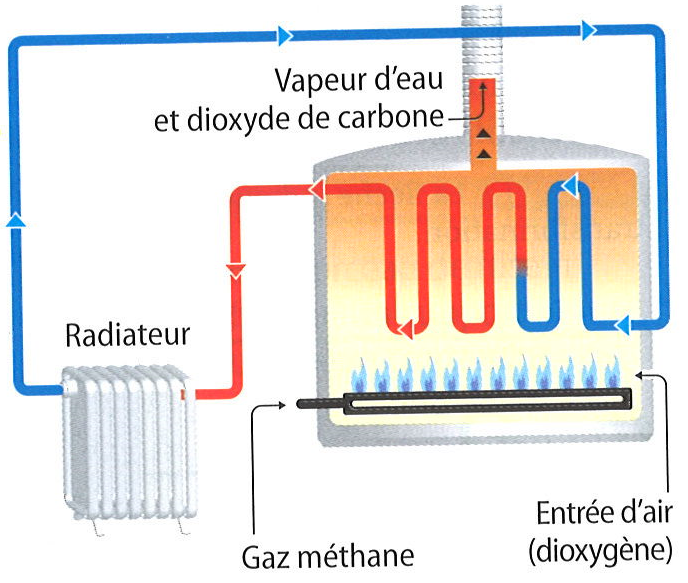
\includegraphics[scale=0.35]{methane}
		\end{center}
	\end{multicols}
\end{doc}

\newpage


\begin{questions}
	\question Quelle est la différence entre un atome et une molécule ?
	
	\fillwithdottedlines{1.5cm}
	
	
	\question 
	
		\begin{parts}
		
			\part Quelle est la formule de la molécule de méthane ?
		
			\fillwithdottedlines{1cm}
			
			\part De quels atomes est elle composée ?
			
			\fillwithdottedlines{1cm}
		\end{parts}
	
	\question Mêmes questions pour le dioxygène.
	\fillwithdottedlines{1.5cm}
	
%	\question Mêmes questions pour l'eau.
%	\fillwithdottedlines{1.5cm}
%	
%	\question Mêmes questions pour le dioxyde de carbone.
%	\fillwithdottedlines{1.5cm}
%	
%	
	\question Dans une réaction chimique, quelle est la différence entre un réactif et un produit ?
	
	\fillwithdottedlines{2cm}
	
	\question Quels sont les réactifs et les produits de la combustion du méthane ?
	
	\fillwithdottedlines{1.5cm}
	
	\question \'Ecrire le bilan en toutes lettres de la combustion du méthane sous la forme :\\
	$ \text{r\'eactif 1} + \text{r\'eactif 2} \rightarrow \text{produit 1} + \text{produit 2}$
	
	\fillwithdottedlines{1cm}
	
	\question Dans ce bilan, remplacer les noms des réactifs et des produits par leur formule ?
	
	\fillwithdottedlines{1cm}
	
	\question Dans les réactifs, combien y a-t-il d'atomes de carbone, d'hydrogène et d'oxygène ?
	
	\fillwithdottedlines{1.5cm}
	
	\question Et dans les produits ?
	
	\fillwithdottedlines{1.5cm}
	
	\question L'équation de réaction est-elle équilibrée ?
	
	\fillwithdottedlines{1cm}
	
	\question Rajouter des coefficients devant les formules des molécules pour obtenir l'équilibre.
	
		\fillwithdottedlines{1cm}
	
\end{questions}


\section{Atomes et molécules}

Parmi les formules suivantes, entourer celles qui désignent des atomes et souligner les molécules.

\begin{multicols}{3}
	\begin{itemize}
		\item $CO_2$
		\item $Fe$
		\item $H_2O$
		\item $H$
		\item $CuSO_4$
		\item $He$
		\item $C_6H_8O_6 $
		\item $Pb$
		\item $NaCl$
		
	\end{itemize}
\end{multicols}


\section{Equations de réaction}

\'Equilibrer les équations des réactions suivantes :

\begin{parts}
	\part \ce{C7H16 + O2 -> CO2 + H2O}
	
	\fillwithdottedlines{1cm}
	
	\part \ce{C4H10 + O2 -> CO2 + H2O}
	
	\fillwithdottedlines{1cm}
	
	\part \ce{C6H2O + O2 -> CO2 + H2O}
	
	\fillwithdottedlines{1cm}
	
	\part \ce{Fe + O2 -> Fe2O3}
	
	\fillwithdottedlines{1cm}
	
	\part \ce{NaBr + Cl2 -> NaCL + Br2}
	
	\fillwithdottedlines{1cm}
	
	\part \ce{Cr2O3 + Mg -> Cr + MgO}
	
	\fillwithdottedlines{1cm}
	
	\part \ce{Mg + HCl -> MgCl2 + H2}
	
	\fillwithdottedlines{1cm}
\end{parts}
	
	

\ \label{LastPage}

\end{document}